\documentclass[11pt,letterpage, fleqn]{article}
\usepackage[lmargin=1in,rmargin=1in,tmargin=1in,bmargin=1in]{geometry}

% -------------------
% Packages
% -------------------
\usepackage{
	amsmath,			% Math Environments
	amssymb,			% Extended Symbols
	enumerate,		% Enumerate Environments
	graphicx,			% Include Images    
	lastpage,			% Reference Lastpage
	multicol,			% Use Multi-columns
	multirow,			% Use Multi-rows
	siunitx
}

\graphicspath{{./images/}}

\usepackage{wrapfig}

% -------------------
% Font
% -------------------
\usepackage[T1]{fontenc}
\usepackage{charter}    


% -------------------
% Heading Commands
% -------------------
\newcommand{\class}{Mu Alpha Theta}
\newcommand{\term}{2022-2023}
\newcommand{\head}[4]{%
\thispagestyle{empty}
\vspace*{-0.5in}
\noindent\begin{tabular*}{\textwidth}{l @{\extracolsep{\fill}} r @{\extracolsep{6pt}} l}
	\textbf{#1} & \textbf{Name:} & \makebox[5.75cm]{\hrulefill} \\
	\textbf{#2} & & \\
	\textbf{\class:\; \term} & & \\
\end{tabular*} \\
\rule[2ex]{\textwidth}{2pt} %
}


% -------------------
% Commands
% -------------------
\newcommand{\prob}{\noindent\textbf{Problem. }}
\newcounter{problem}
\newcommand{\problem}{
	\stepcounter{problem}%
	\noindent \textbf{Problem \theproblem. }%
}
\newcommand{\pointproblem}[1]{
	\stepcounter{problem}%
	\noindent \textbf{Problem \theproblem.} (#1 points)\,%
}
\newcommand{\pspace}{\par\vspace{\baselineskip}}
\newcommand{\ds}{\displaystyle}


% -------------------
% Header & Footer
% -------------------
\usepackage{fancyhdr}

\fancypagestyle{pages}{
	%Headers
	\fancyhead[L]{}
	\fancyhead[C]{}
	\fancyhead[R]{}
\renewcommand{\headrulewidth}{0pt}
	%Footers
	\fancyfoot[L]{}
	\fancyfoot[C]{}
	\fancyfoot[R]{}
\renewcommand{\footrulewidth}{0.0pt}
}
\headheight=0pt
\footskip=14pt

\pagestyle{pages}


% -------------------
% Content
% -------------------

\begin{document}
\head{Worksheet \#7}{Date: December 5th, 2022}
\centering

% Question 1: 768 (2004 AMC10A p12) https://artofproblemsolving.com/wiki/index.php/2004_AMC_10A_Problems/Problem_12
\begin{minipage}{\textwidth}
	\problem

   \noindent Henry's Hamburger Haven offers its hamburgers with the following condiments: ketchup, mustard, mayonnaise, tomato, lettuce, pickles, cheese, and onions. A customer can choose one, two, or three meat patties and any collection of condiments. How many different kinds of hamburgers can be ordered?

    \vspace{2cm}
\end{minipage}

% Question 2: pi/7 (2004 AMC10A p21) https://artofproblemsolving.com/wiki/index.php/2004_AMC_10A_Problems/Problem_21
\begin{minipage}{\textwidth}
    \problem

	\begin{wrapfigure}[11]{l}{0.4\textwidth}
		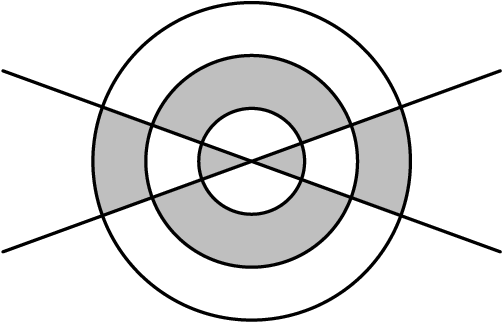
\includegraphics[width = 4cm]{p21-2004.png}
   \end{wrapfigure}
   \noindent Two distinct lines pass through the center of three concentric circles of radii 3, 2, and 1. The area of the shaded region in the diagram is $\frac{8}{13}$ of the area of the unshaded region. What is the radian measure of the acute angle formed by the two lines? (Note: $\pi$ radians is $180$ degrees.)
	
   \vspace{4cm}
\end{minipage}

% Question 3: 240 (2004 AMC10A p19) https://artofproblemsolving.com/wiki/index.php/2004_AMC_10A_Problems/Problem_19
\begin{minipage}{\textwidth}
    \problem

	\begin{wrapfigure}[11]{r}{0.3\textwidth}
		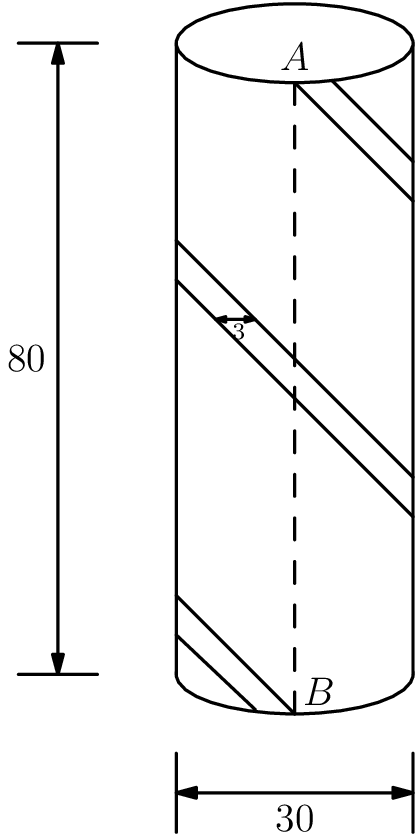
\includegraphics[width = 4cm]{p19-2004.png}
   \end{wrapfigure}
   \noindent A white cylindrical silo has a diameter of 30 feet and a height of 80 feet. A red stripe with a horizontal width of 3 feet is painted on the silo, as shown, making two complete revolutions around it. What is the area of the stripe in square feet?

   \vspace{7cm}
\end{minipage}

% Question 4: 8/9 (2004 AMC10A p23) https://artofproblemsolving.com/wiki/index.php/2004_AMC_12A_Problems/Problem_19
\begin{minipage}{\textwidth}
    \problem

	\begin{wrapfigure}[11]{r}{0.3\textwidth}
		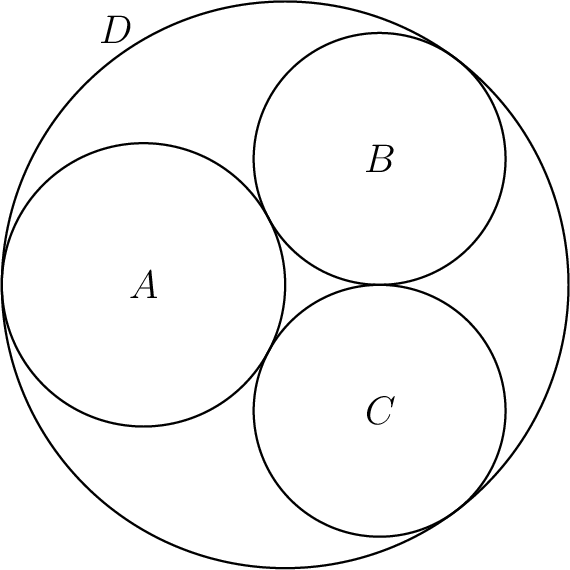
\includegraphics[width = 4cm]{p23-2004.png}
   \end{wrapfigure}
   \noindent Circles $A, B$ and $C$ are externally tangent to each other, and internally tangent to circle $D$. Circles $B$ and $C$ are congruent. Circle $A$ has radius $1$ and passes through the center of $D$. What is the radius of circle $B$?

   \vspace{8cm}
\end{minipage}

% Question 5: 3 + √(69)/3 (2004 AMC10A p25) https://artofproblemsolving.com/wiki/index.php/2004_AMC_12A_Problems/Problem_22
\begin{minipage}{\textwidth}
    \problem

   \noindent Three mutually tangent spheres of radius $1$ rest on a horizontal plane. A sphere of radius $2$ rests on them. What is the distance from the plane to the top of the larger sphere?

   \vspace{7cm}
\end{minipage}

\vspace{6cm}
\end{document}

